\chapter{Model 3D}
\label{cha:model}

Ostatnim etapem projektu było zaprojektowanie słuchawek w formie modelu trójwymiarowego. Użyto do tego celu programu \textit{Autodesk Inventor Professional 2018}, wykorzystując licencję studencką. 

Na końcowe złożenie całości składają się pliki oddzielne dla każdego komponentu. Projektując poszczególne elementy, brano pod uwagę możliwość wydruku na drukarce 3D, a więc nie stosowano cienkich, ani wiszących elementów. Szkice, będące podstawami do brył były wymiarowane i wiązane tak, aby zapewnić możliwość łatwej modyfikacji. Muszle słuchawek mają kształt elips o wymiarach $80x100mm$.


\section{Słuchawka lewa}
\label{cha:model_lewa}

Wycięcie na lewą płytkę PCB zrobiono w wysuniętym elemencie muszli, które w górnej części pokrywa się z pełnymi wymiarami, a w dolnej zostało skrócone o \textbf{WYMIAR} i ścięte pod kątem $45^{\circ}$. Powodem był kształt płytki i umiejscowienie przycisków, z których główny jest obrócony pod takim kątem w stosunku do reszty.

Na horyzontalnej ściance umieszczono przyciski \textbf{plus} i \textbf{minus} oraz otwór na kabel do radiotelefonu, natomiast pod katem główny przycisk oraz otwór na pałąk do mikrofonu komunikacyjnego.

Muszla ma w samym centrum elipsy otwór, umożliwiający akwizycję dźwięków przez mikrofon, który również wymierzono tak, aby znajdował się w centralnym punkcie.

\begin{figure}[H]
	\centering
	\begin{subfigure}{.45\textwidth}
		\centering
		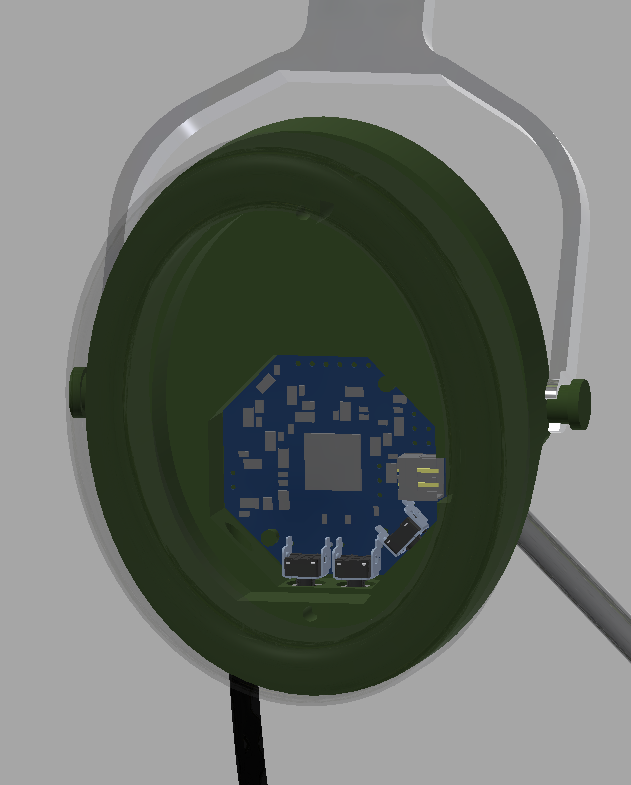
\includegraphics[height=7cm]{zdjecia/model/left_in.png}
		\subcaption{Strona wewnętrzna}
	\end{subfigure}
	\begin{subfigure}{.45\textwidth}
		\centering
		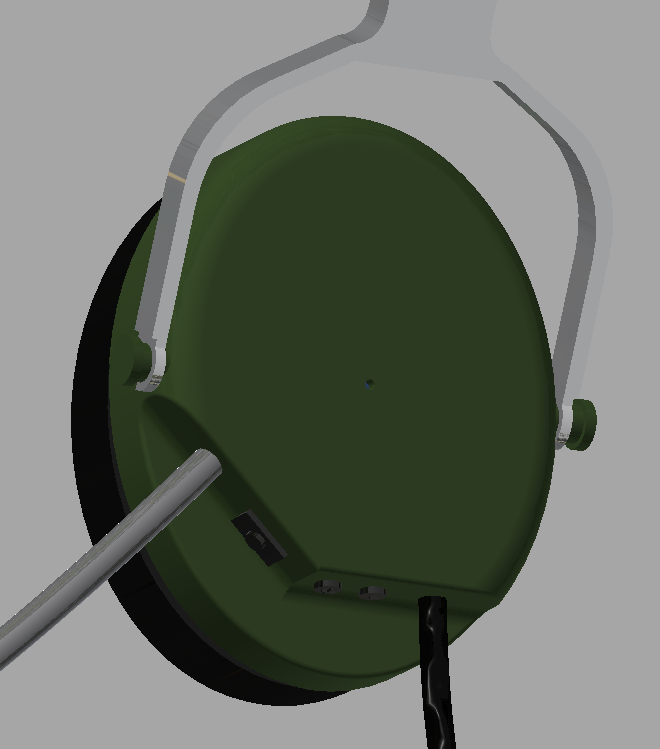
\includegraphics[height=7cm]{zdjecia/model/left_out.png}
		\subcaption{Strona zewnętrzna}
	\end{subfigure}
	\caption{\label{pic:lewa_sluchawka} Model 3D lewej słuchawki}
\end{figure}


\section{Słuchawka prawa}
\label{cha:model_prawa}

Model prawej muszli jest zewnętrznie lustrzanym odbiciem lewej. Różni się otworami na dolnych ściankach wypustu w obudowie. Tutaj zastosowany tylko jeden, pozwalający podłączyć kabel mikro USB. Na zewnętrznej ściance zrobiono dodatkowo niewielki otwór w kształcie baterii, przez który widać światło diody LED, wskazującej stan ładowania słuchawek.

Miejsce na płytkę PCB zostało dostosowane do montażu płytki lewej według wymiarów layoutu i umiejscowione tak, aby port mikrofonu znajdował się na samym środku słuchawki.

\begin{figure}[H]
	\centering
	\begin{subfigure}{.45\textwidth}
		\centering
		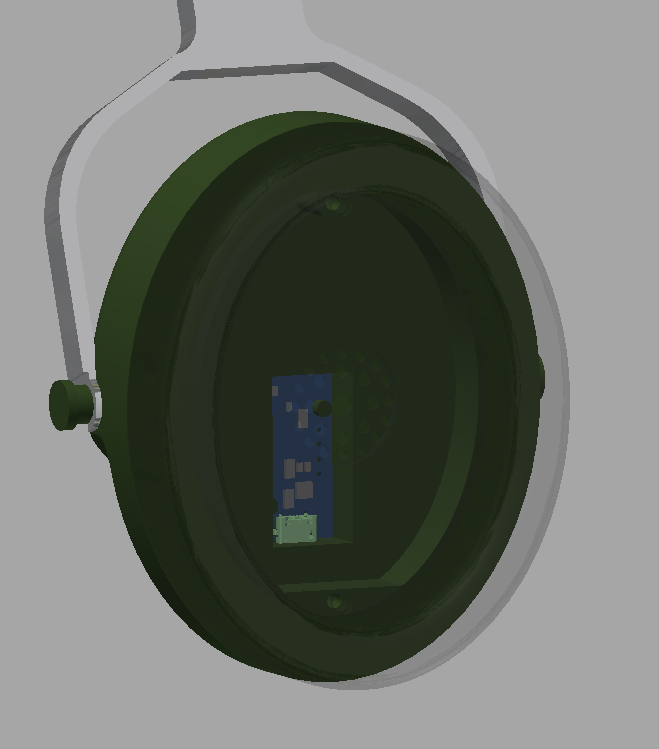
\includegraphics[height=7cm]{zdjecia/model/right_in.png}
		\subcaption{Strona wewnętrzna}
	\end{subfigure}
	\begin{subfigure}{.45\textwidth}
		\centering
		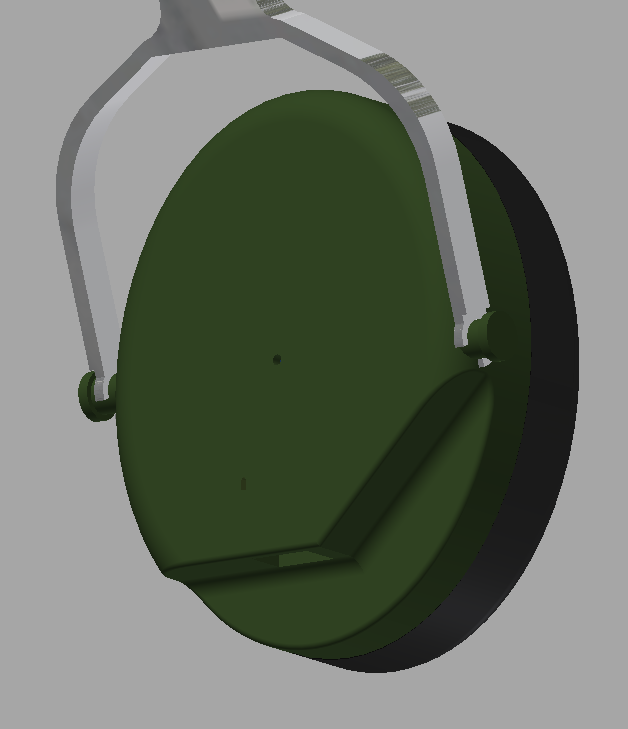
\includegraphics[height=7cm]{zdjecia/model/right_out.png}
		\subcaption{Strona zewnętrzna}
	\end{subfigure}
	\caption{\label{pic:prawa_sluchawka} Model 3D prawej słuchawki}
\end{figure}


\section{Pałąk}
\label{cha:model_palak}

Pałąk słuchawek stworzono na planie okręgu o średnicy $200mm$. Każda ze słuchawek ma dodatkowo własny mały pałąk, który jest montowany na obrotowych zawiasach do muszli oraz wsuwany do głównego pałąku, umożliwiając dostosowanie wysokości do głowy użytkownika.

\begin{figure}[H]
	\centering
	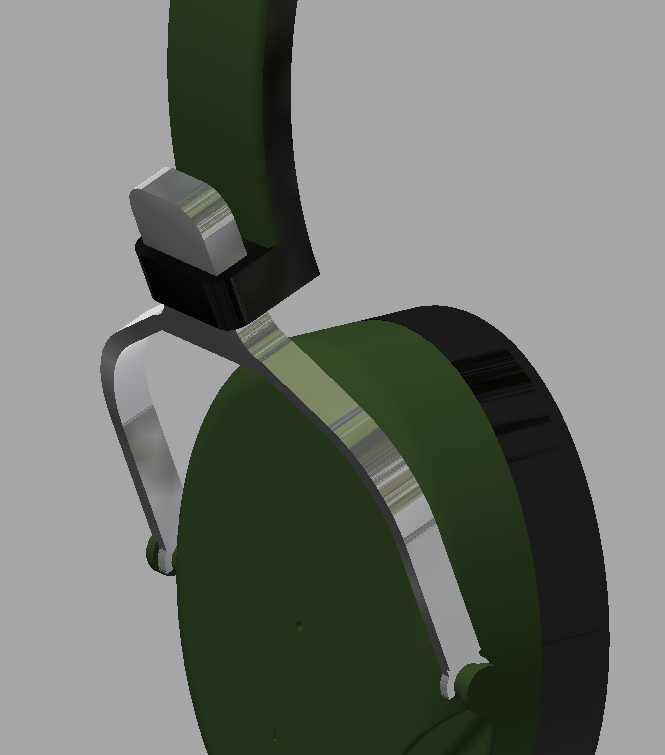
\includegraphics[height=7cm]{zdjecia/model/hinge.png}
	\caption{\label{pic:hinge}Zawias lewej słuchawki}
\end{figure}